\documentclass[a4paper, 10pt]{article}
\usepackage[utf8]{inputenc} % Change according your file encoding
\usepackage{graphicx}
\usepackage{url}

%opening
\title{Seminar Report: Chordy}
\date{\normalsize\today{}}

\begin{document}
\author{}
\maketitle

\begin{center}
  \textbf{Carles Tornel}\\
  \textbf{Jesus Alfaro}\\
  \textbf{Ricard Abril}

\end{center}
\section{Introduction}
En aquesta pràctica implementarem una hash table distribuida d'acord amb l'esquema Chord. Primerament podrem afegir nodes i posteriorment afegirem l'opció de tenir storage i controlar la caiguda d'un node així com recuperar storage.

\newpage\section{Experiments}
\subsection{Building a Ring}
\subsubsection{Do some experiments to test the ring integrity, initially in one Erlang instance but then in a network of several instances. When con- necting nodes on different instances remember to start Erlang in distributed mode (giving a -name argument) and make sure that you use the same cookie (-setcookie).}
En aquest punt, el nostre codi, és capaç de crear un ring i afegir-ne nodes.\\ 
Així que per comprovar que funciona correctament hem creat 4 nodes i hem enviat missatges ha aquest node, per tal de veure si es reben correctament i el temps que triguen a arribar. Tal com podem veure en la imatge següent:\\\\
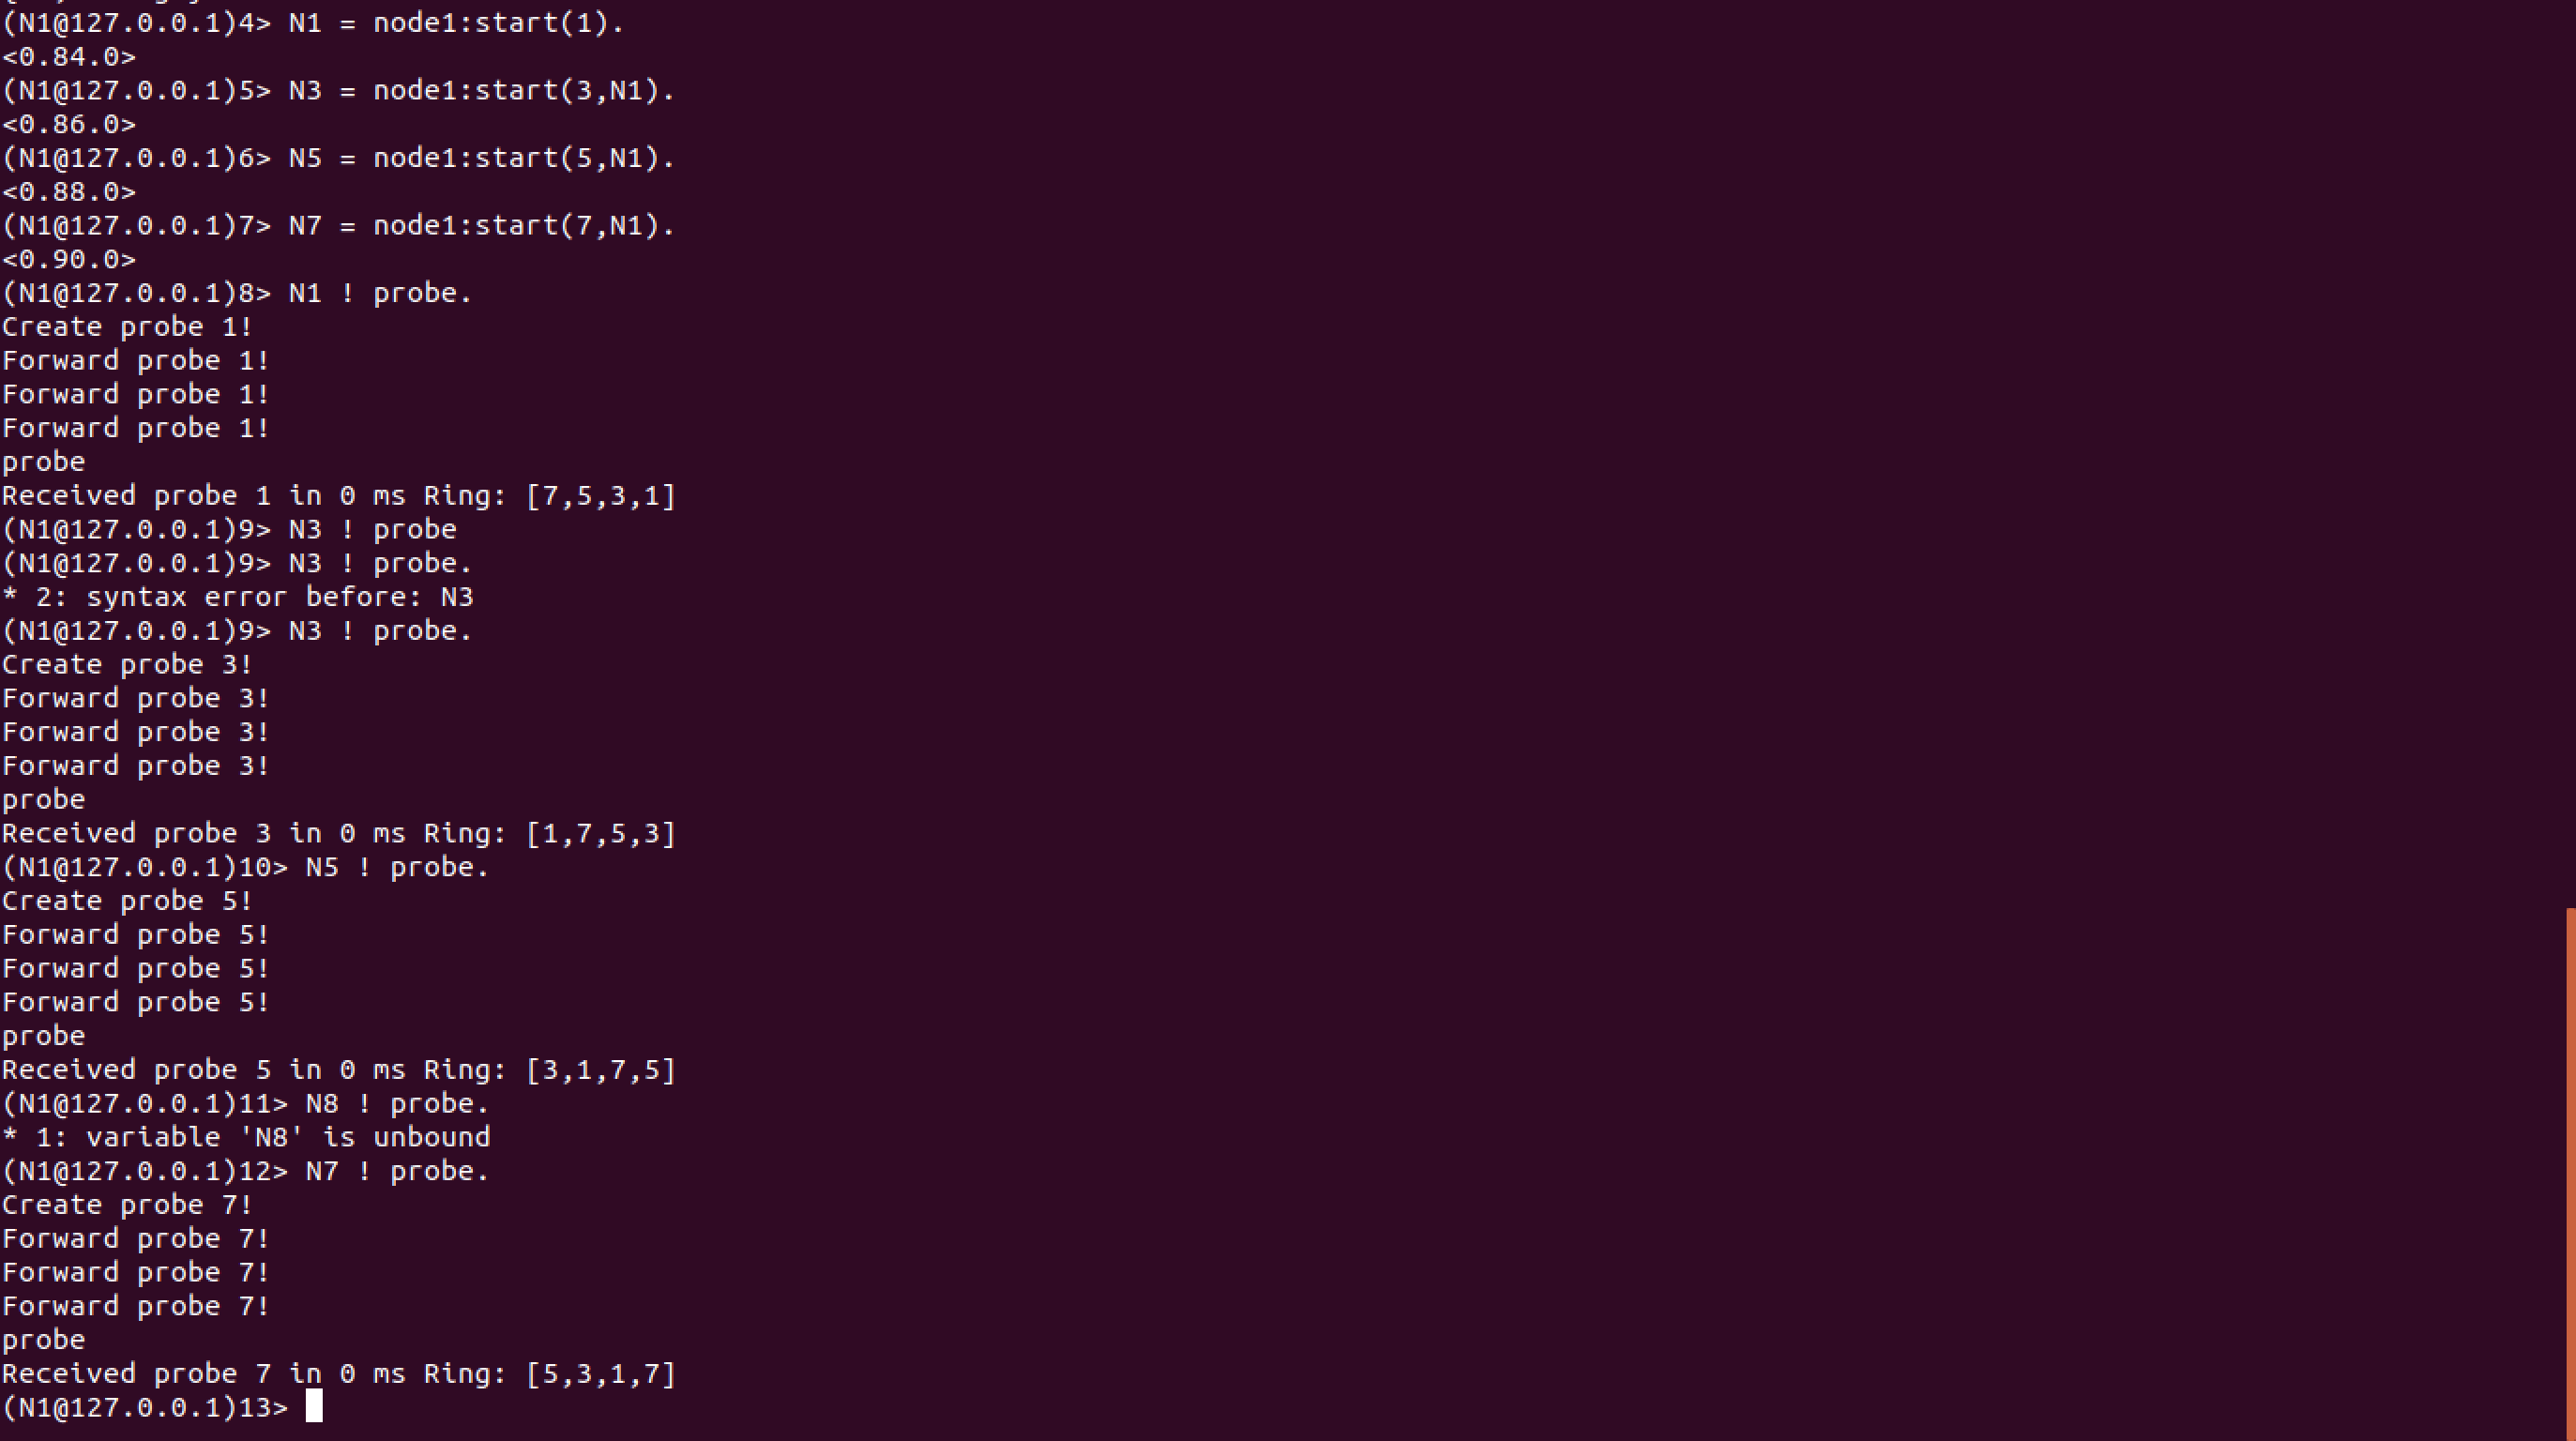
\includegraphics[width=\textwidth]{Ex1.png}
\newpage
\subsection{Adding Store}
\subsubsection{ If we now have a distributed store that can handle new nodes that are added to the ring we might try some performance testing. You need several machines to do this. Assume that we have eight machines and that we will use four in building the ring and four in testing the performance.}

Ara el nostre codi ja és capaç de gestionar un "Storage" en els nodes, de forma que podrem emmagatzemar i buscar elements en forma de clau - valor en ells.\\
Per comprovar que funciona correctament, hem afegit diferents elements als nodes. Tal com podem veure a continuació:\\\\
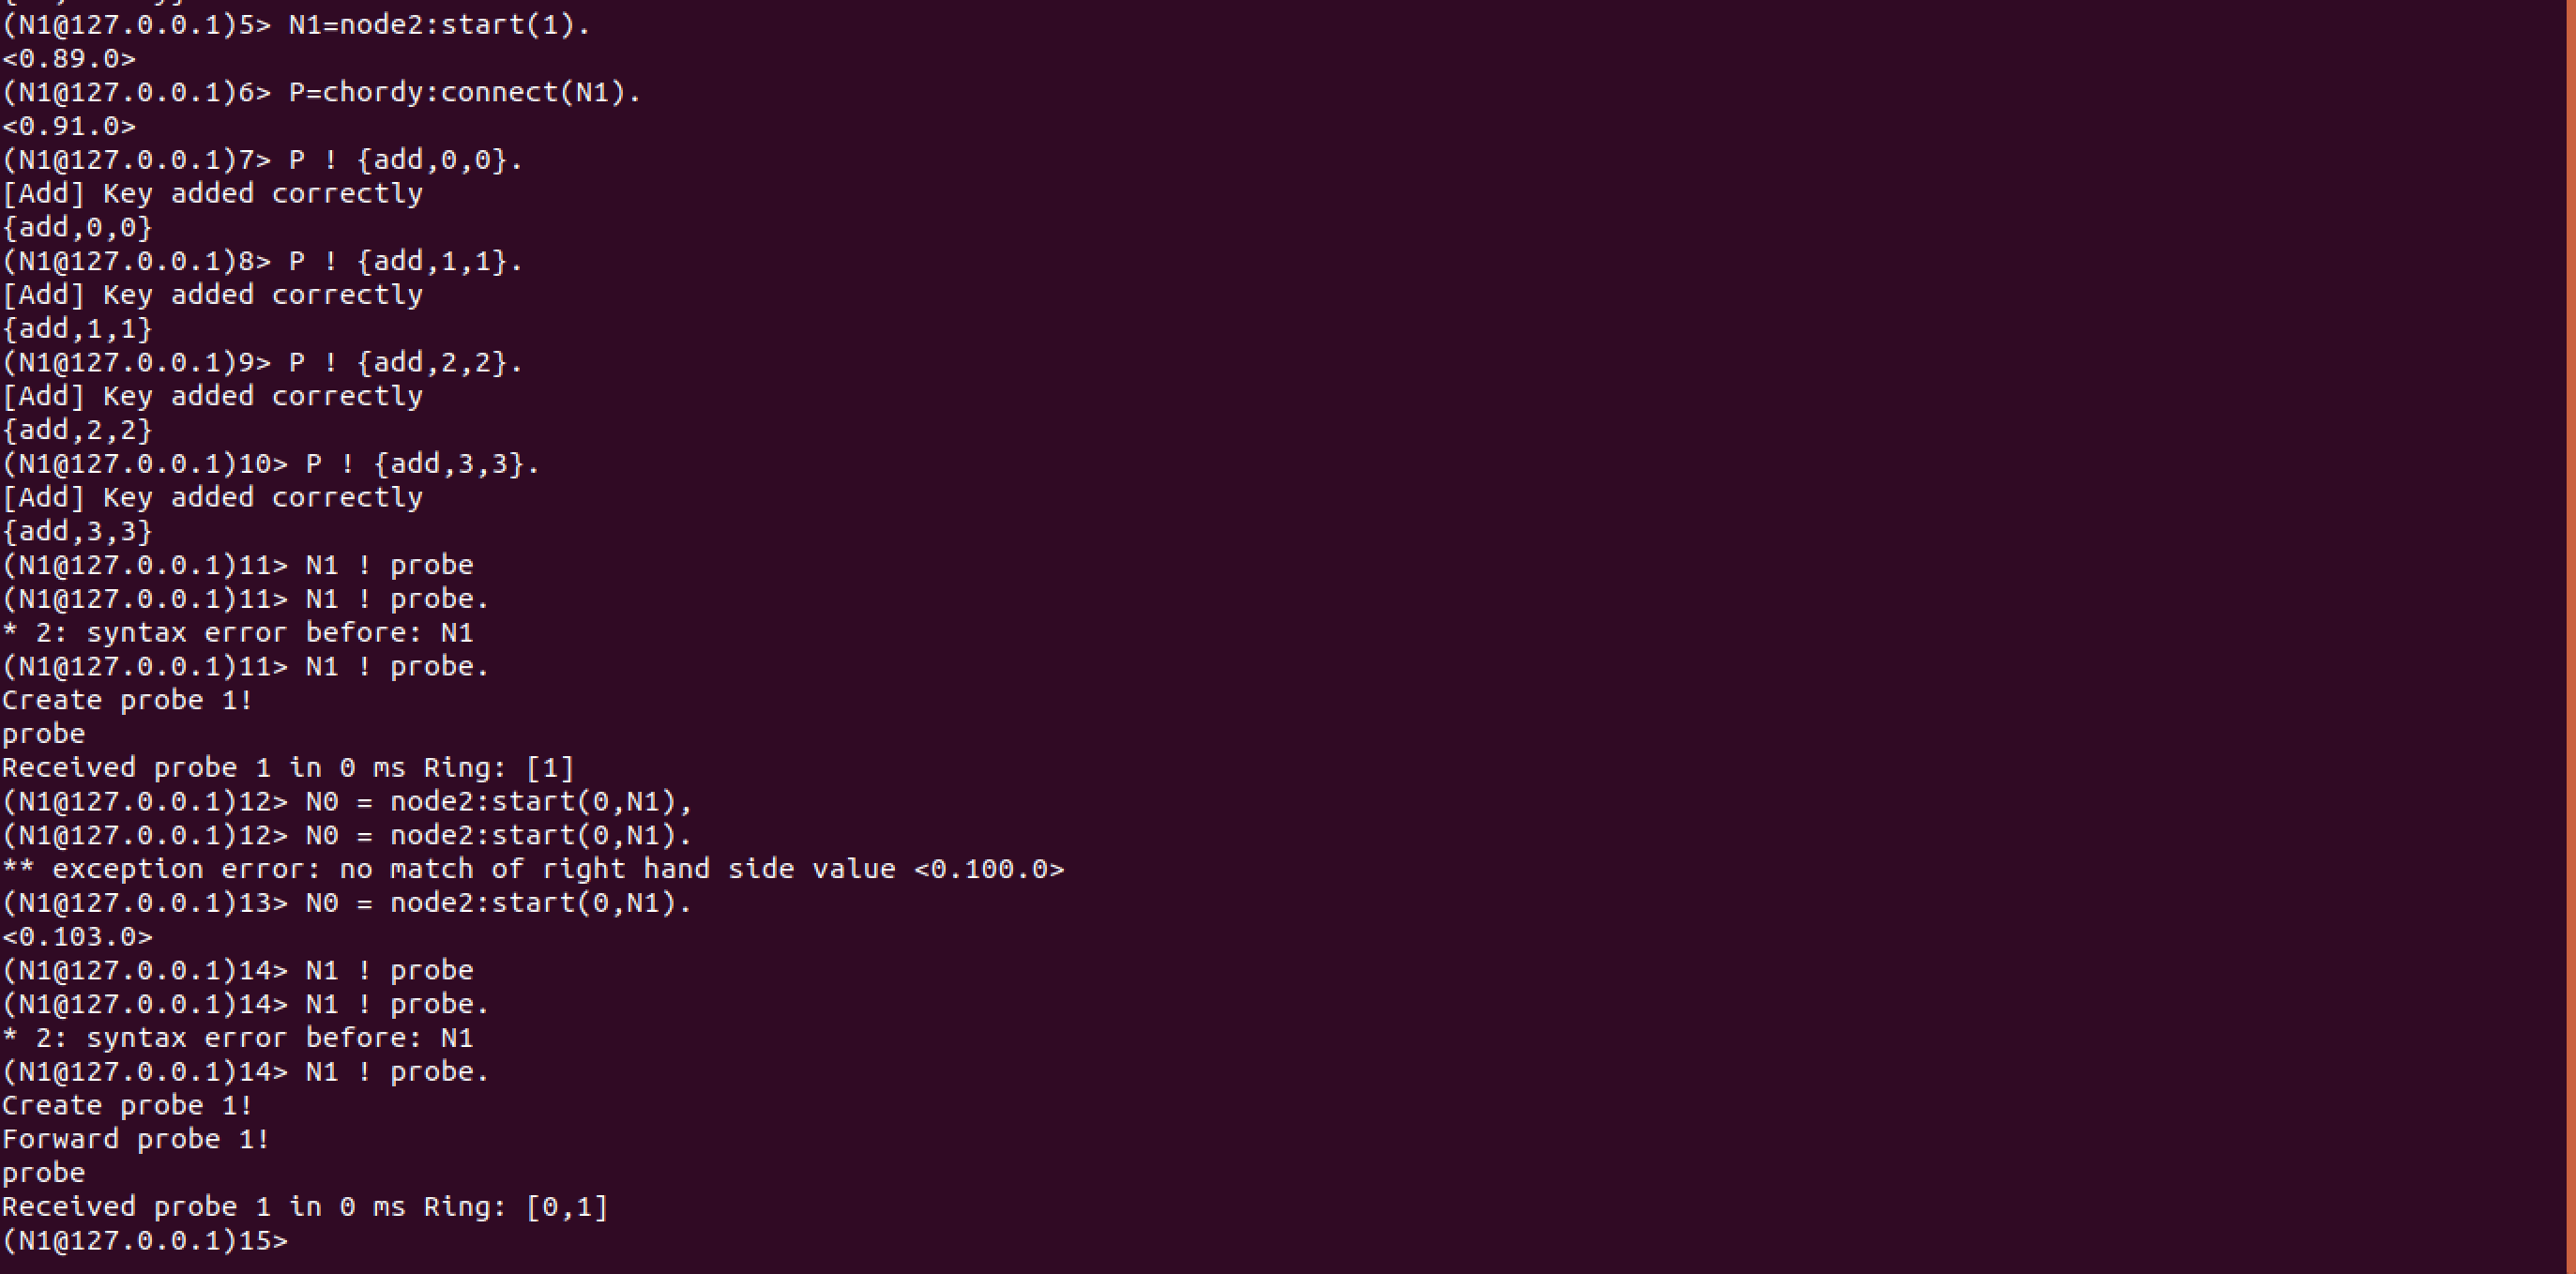
\includegraphics[width=\textwidth]{Ex2.png}

\subsubsection{As a first test, build a ring with one node only and let each of the four test machines add a number (e.g., 1000) of random elements (key-value pairs) to the ring and then do a lookup of the elements, measuring the time it takes. You can use the test procedure given in ’Appendix A’, which should be given with the ID of the node to contact. You should use the function key:generate() to assign the keys of the nodes in the ring, so that elements will get uniformly distributed among them.}

En aquest test, només tindrem un node al ring, al qual afegirem un nombre aleatori d'entrades i comprovarem el seu funcionament mitjançant el codi de prova facilitat en l'apèndix de la pràctica.\\\\
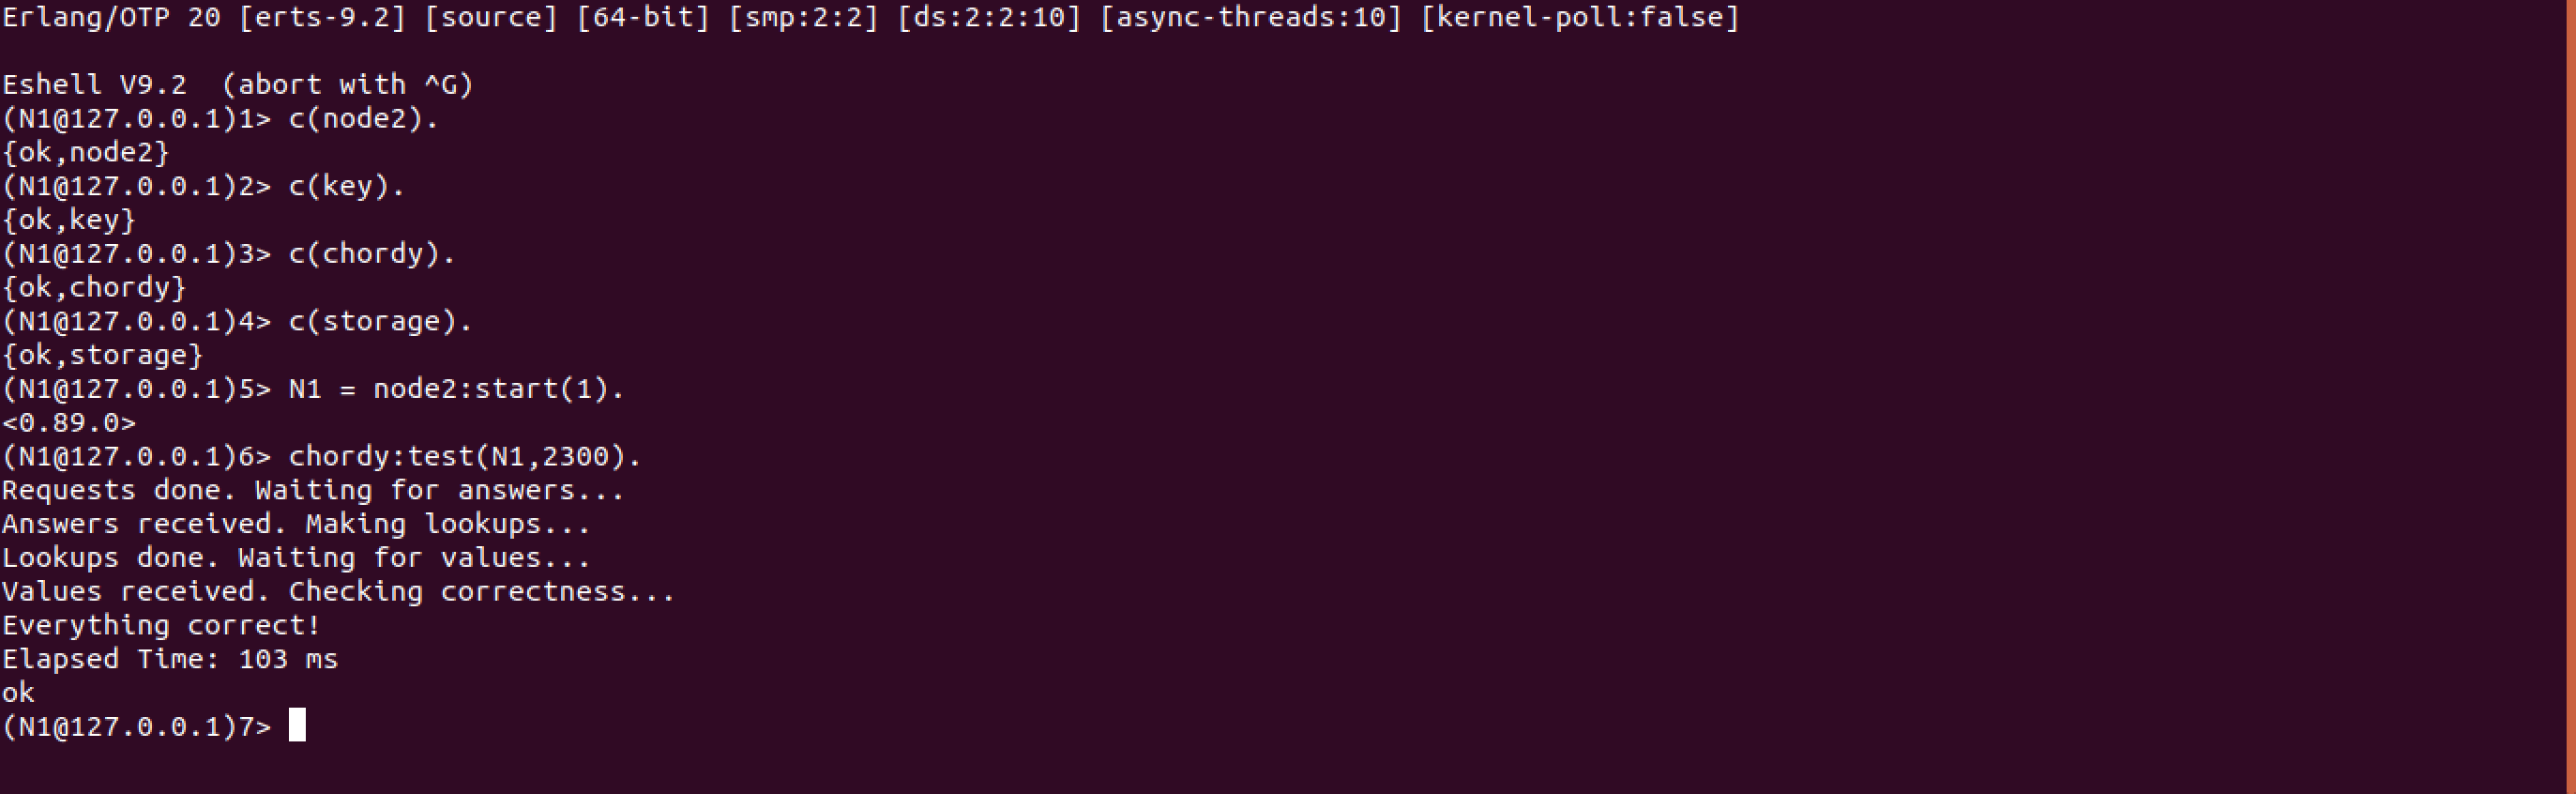
\includegraphics[width=\textwidth]{Ex3.png}

\subsubsection{For the next test, you should add another node to the ring and check how the performance changes. Then, add two more nodes to the ring, any changes? Check also the impact on the performance if all the test machines access the same node or different nodes in the ring.}

En aquest experiment, repetirem el procediment de l'anterior, però afegint més nodes al ring, per tal de veure el canvi de rendiment del sistema.\\
Amb 2 nodes:\\\\
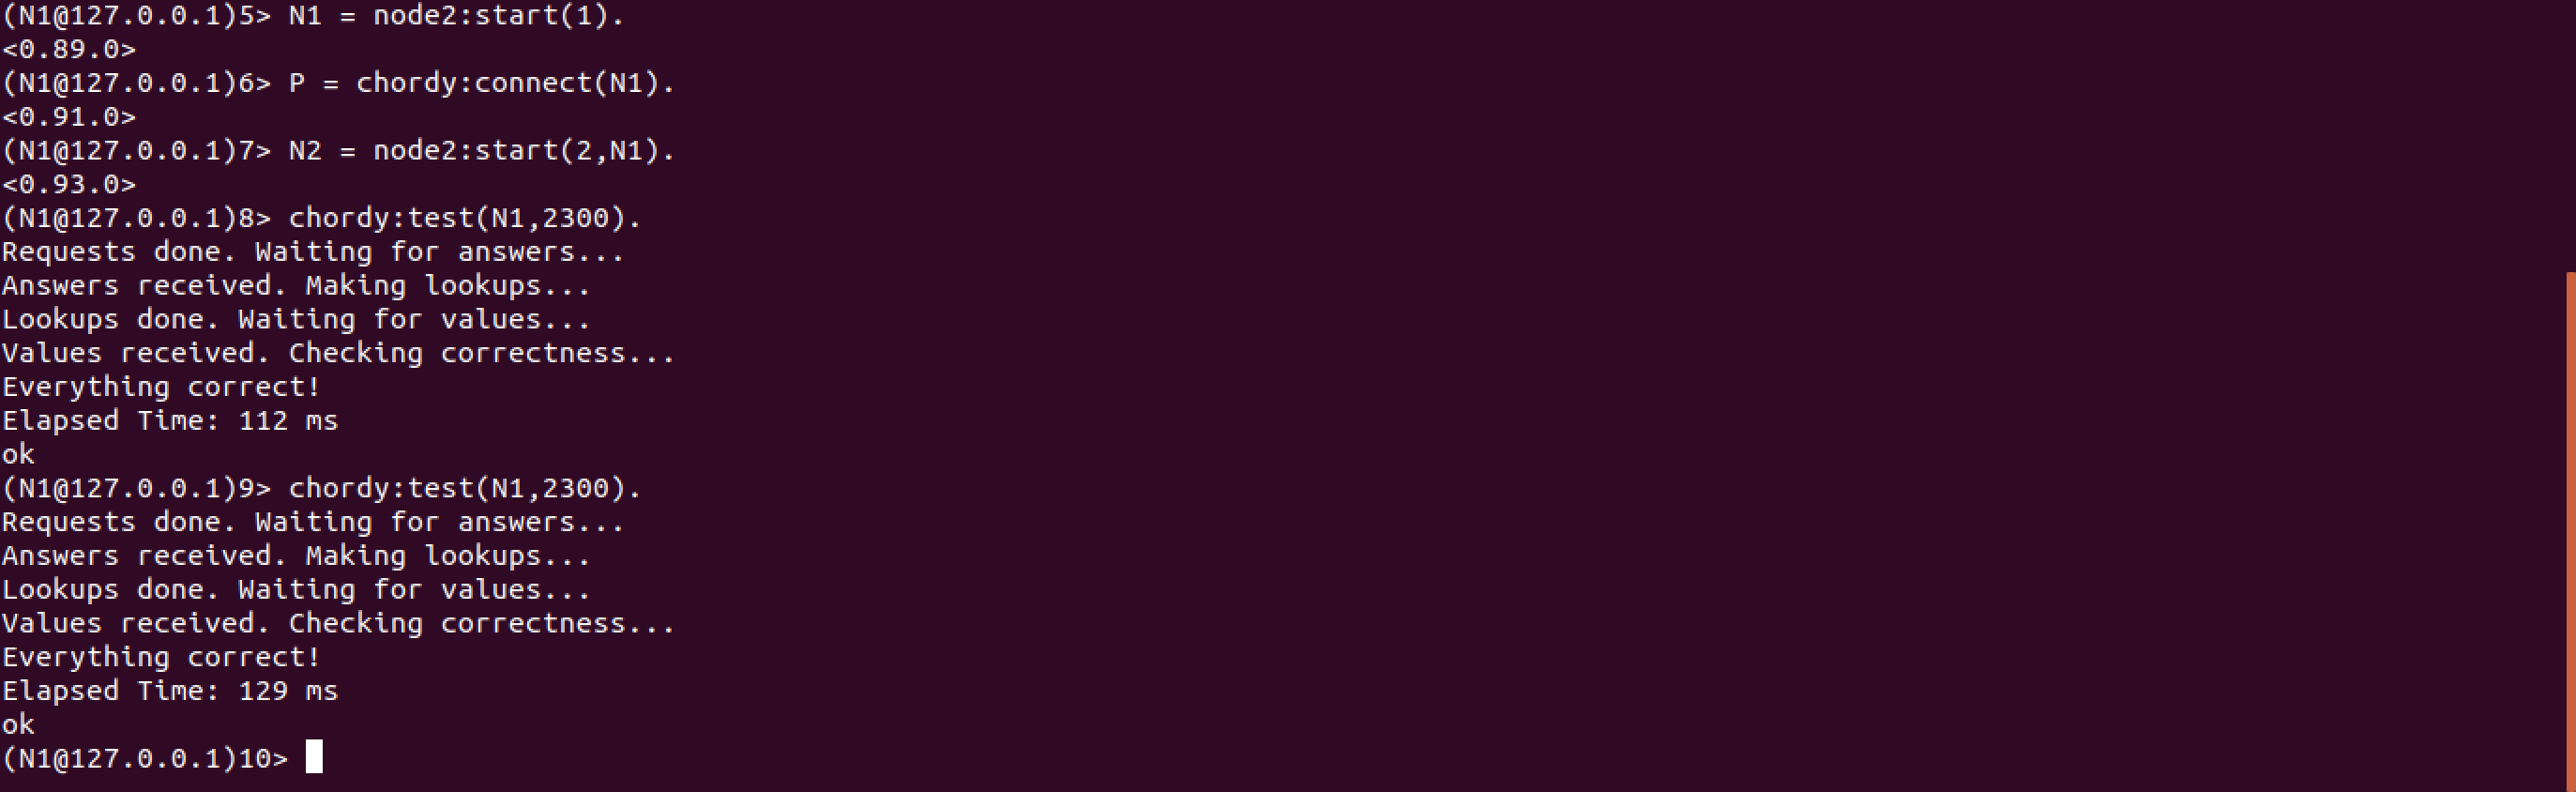
\includegraphics[width=\textwidth]{Ex4.png}\\
Amb 4 nodes:\\\\
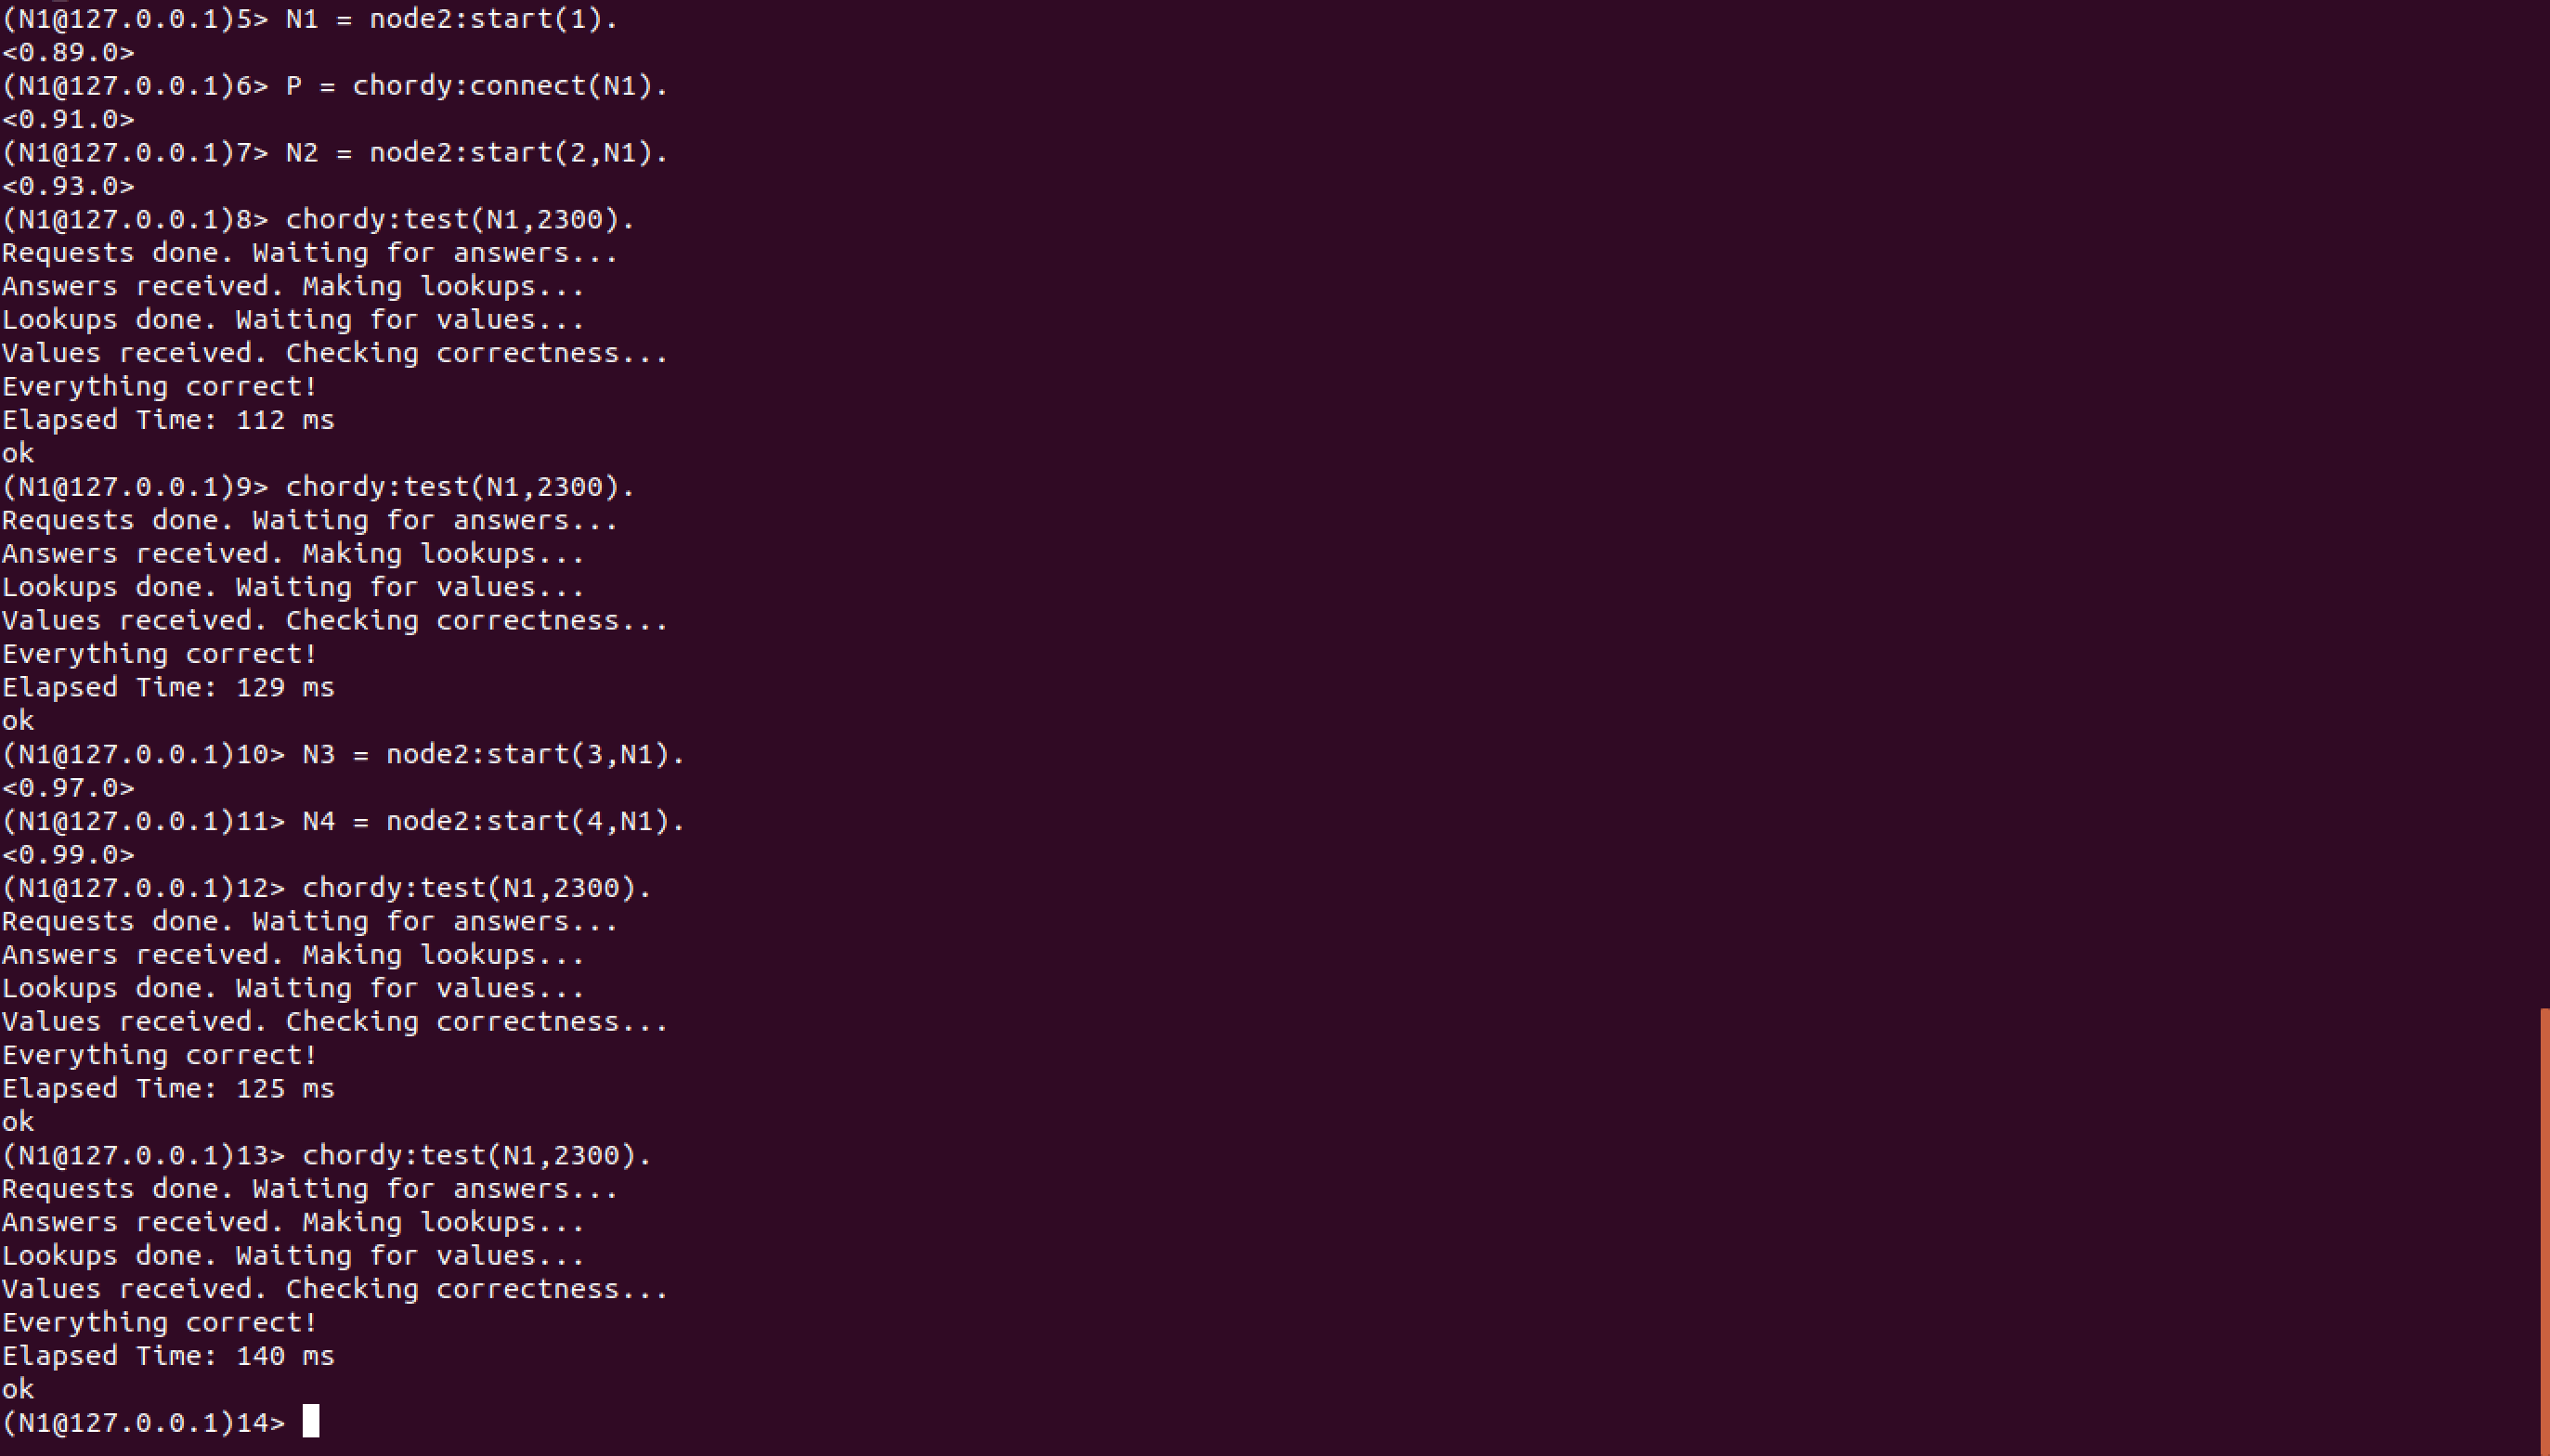
\includegraphics[width=\textwidth]{Ex5.png}
\newpage
\subsection{Handling Failure}
\subsubsection{Experiments. Do some experiments to evaluate the behavior of your implementation when nodes can fail.}

Ara el nostre codi, hauria de ser tolerant a fallades, és a dir que encara que un node caigués el programa que avalua el codi no hauria de donar errors.\\\\
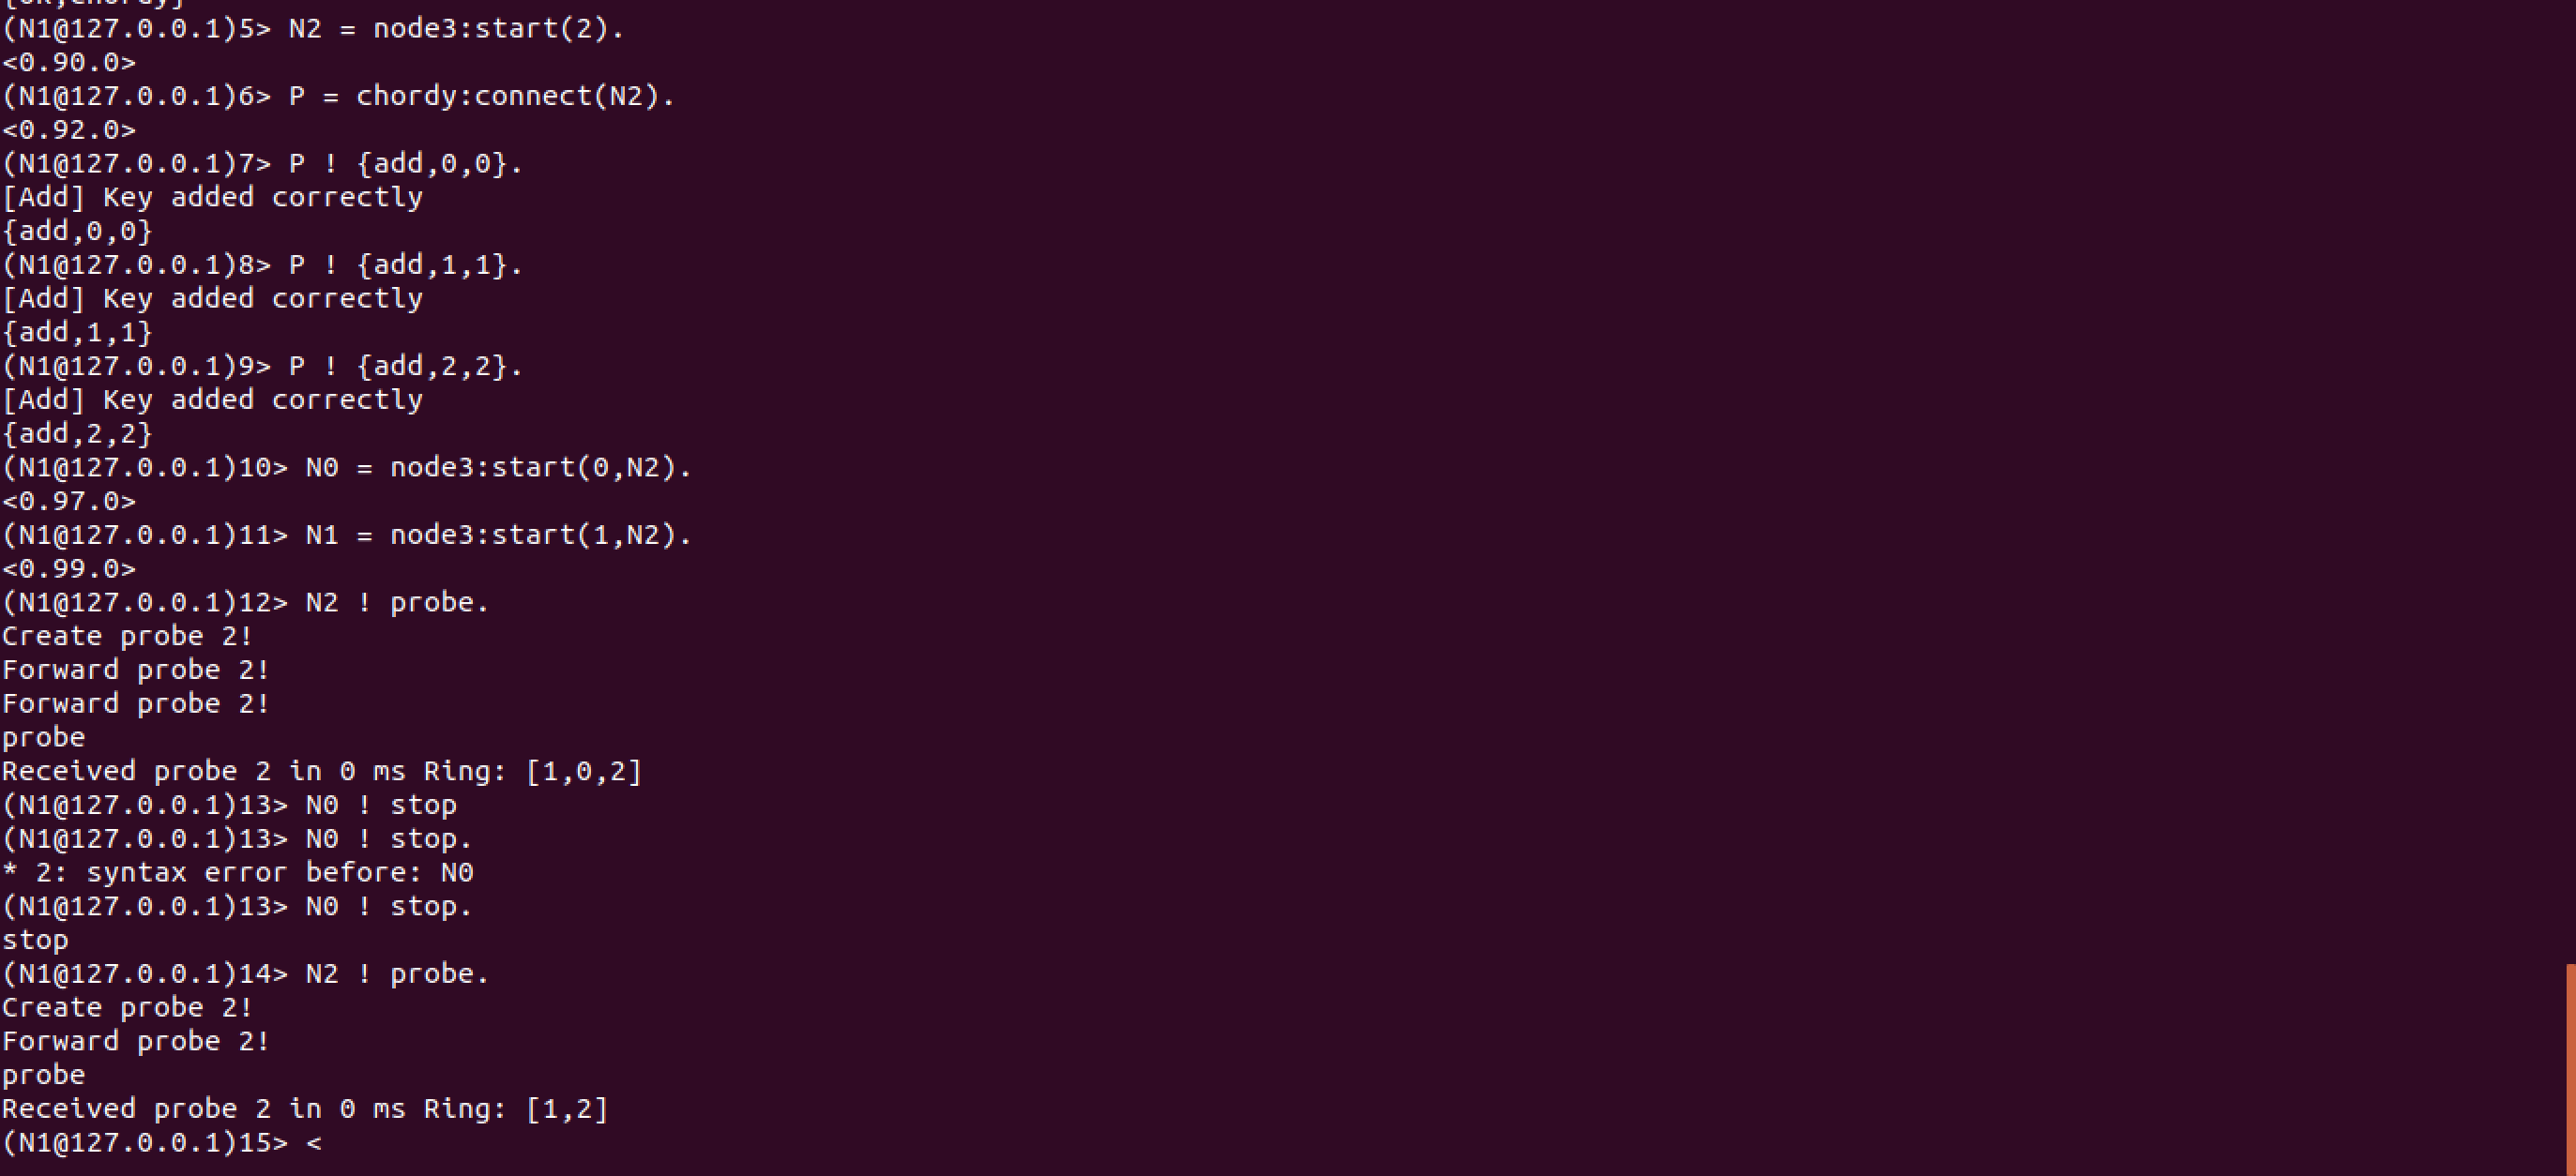
\includegraphics[width=\textwidth]{Ex6.png}

\newpage\subsection{Replication}
\subsubsection{Do some experiments to demonstrate that your replica- tion strategy works. You can for instance execute the following commands, and check the contents of the Store and the Replica.}

En aquesta última implementació, el nostre codi hauria de permetre replicar les entrades d'un node en un altre, per comprovar-ho, utilitzarem el codi donat. Tal com podem veure a continuació.\\\\

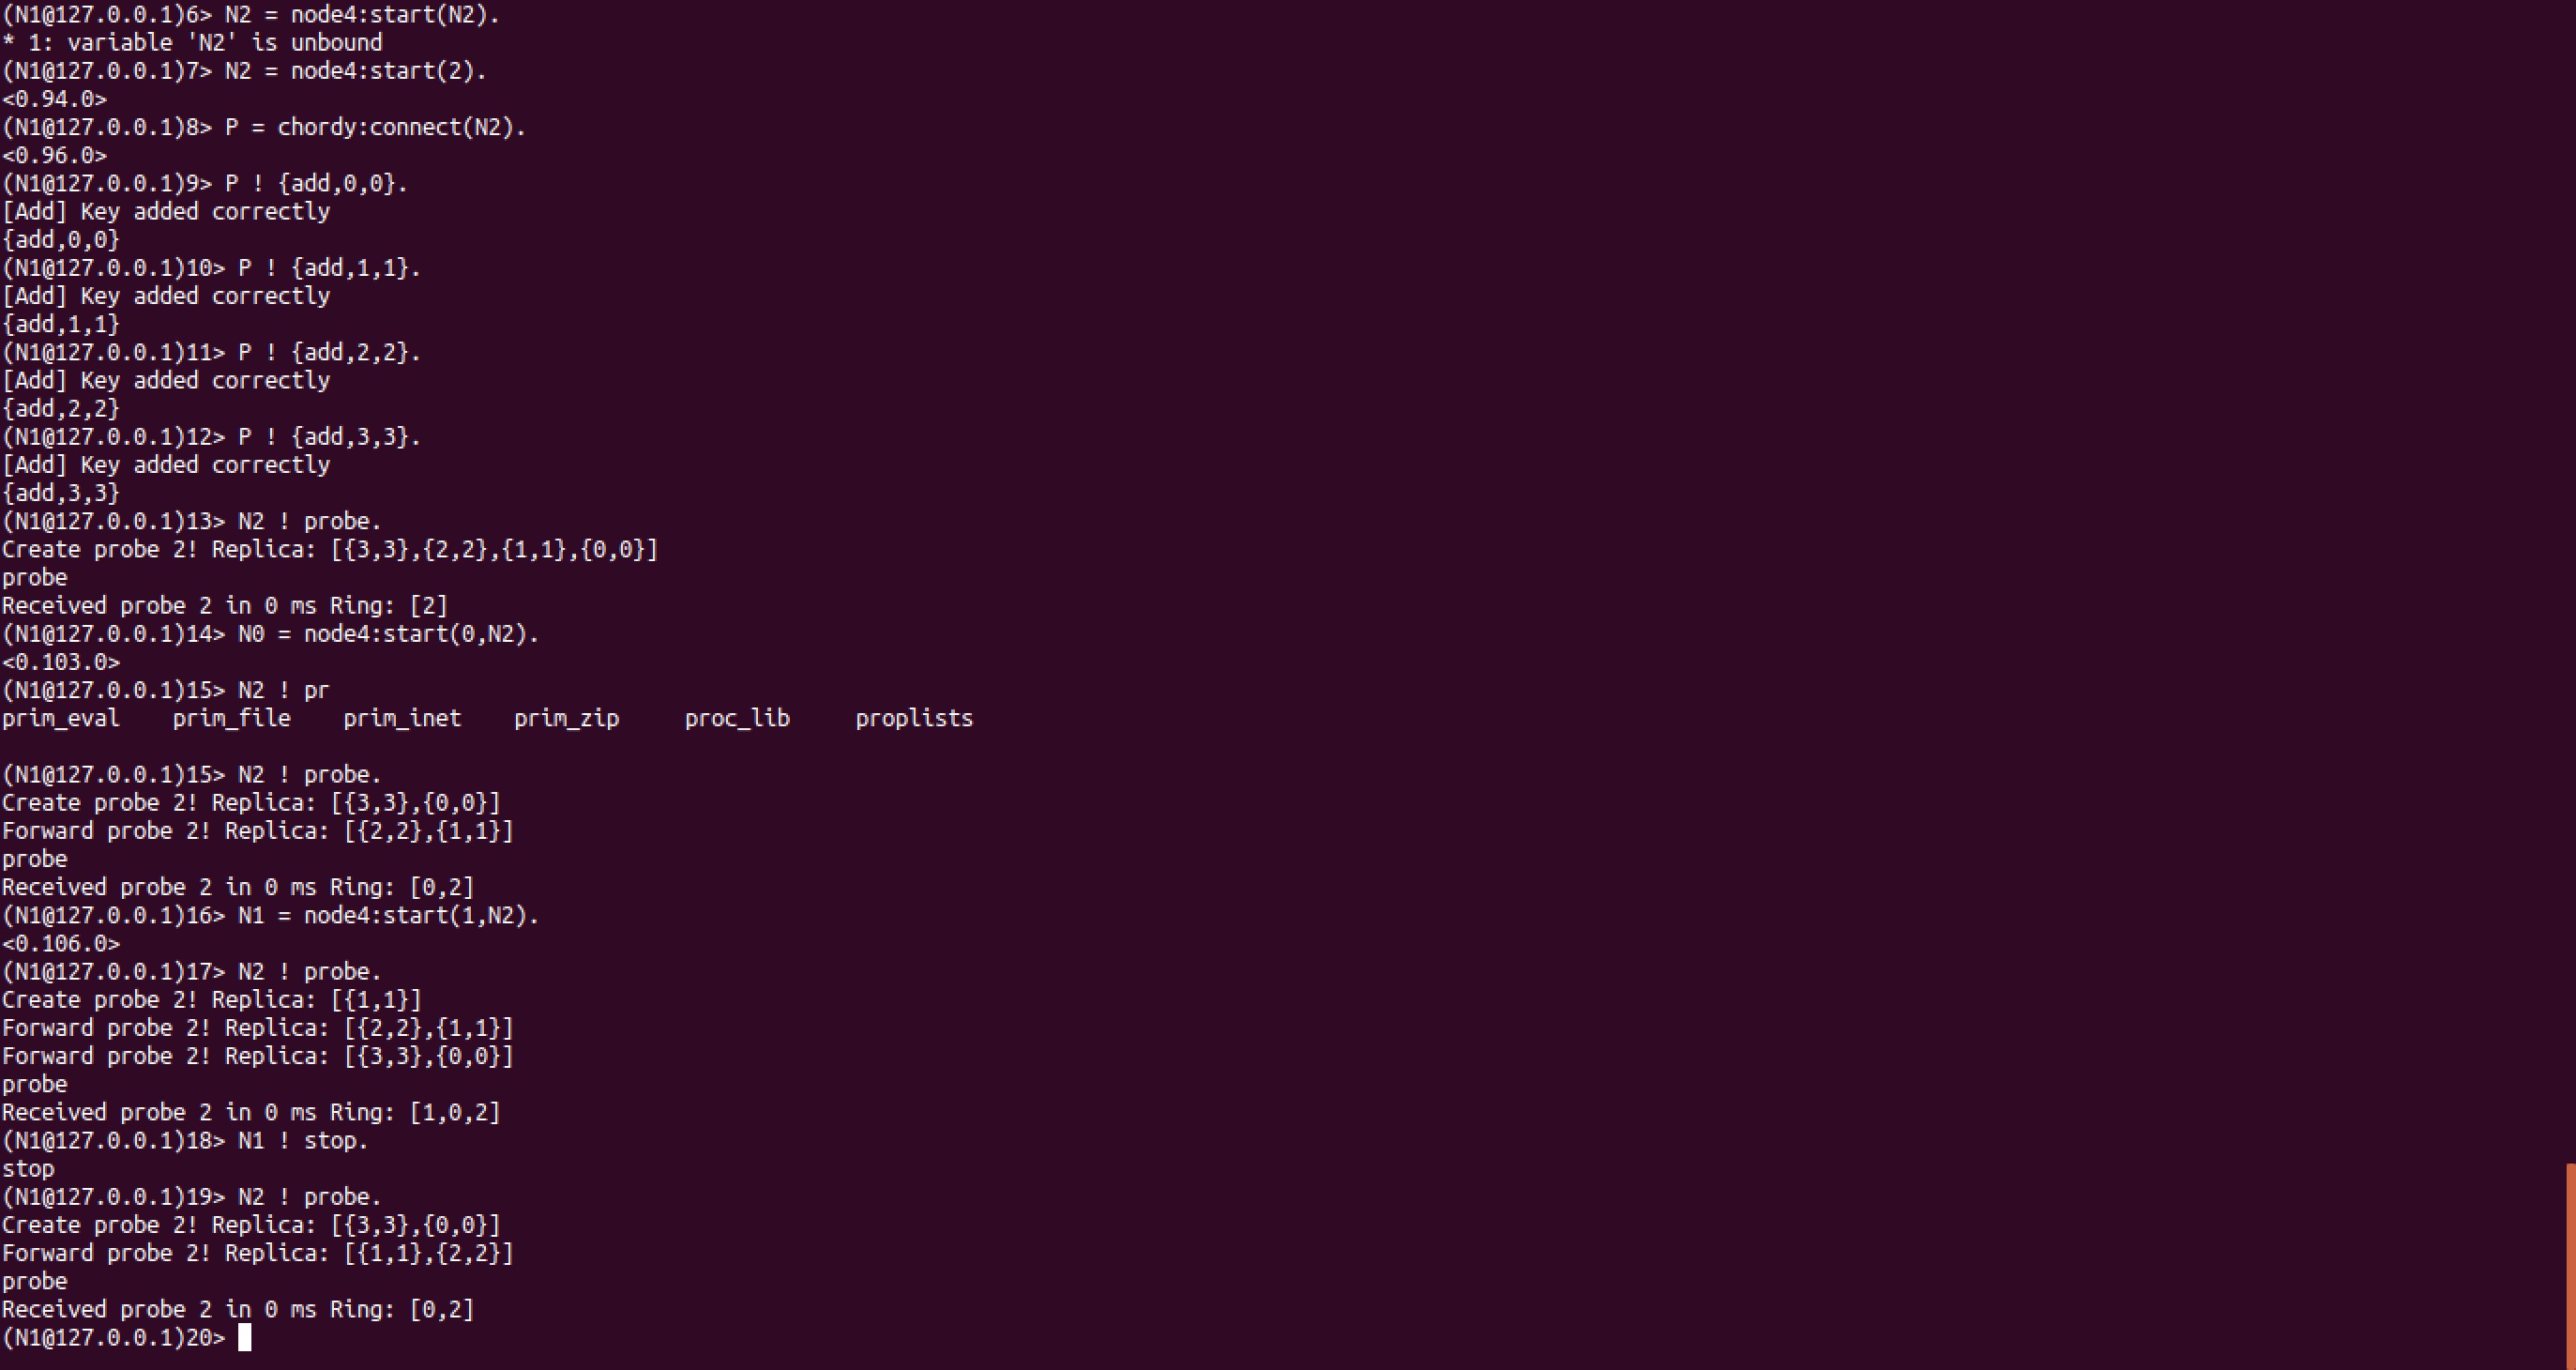
\includegraphics[width=\textwidth]{Ex7.png}
\newpage\section{Open Questions}
\subsection{Building a Ring}
\subsubsection{What are the pros and cons of a more frequent stabilizing procedure?}
Amb una freqüència d'estabilització alta podrem determinar més rapidament quins nodes encara no són estables a l'anell i reduirem l'estat d'inestabilitat a l'anell. Encara que hauríem de tenir en compte si el overhead creat pels missatges d'estabilització és òptim respecte la velocitat d'estabilització dels nodes, ja que no sempre amb un procediment d'estabilització més freqüent s'aconsegueix una millora en la velocitat d'enllaçament dels nodes.
\subsubsection{Do we have to inform the new node about our decision? How will it know if we have discarded its friendly proposal?}
L'haurem d'informar sempre, ja que no tindrà informació suficient per determinar el seu lloc a l'anell per si mateix.
Si no acceptem la seva proposició significa que no pot ser el nostre predecessor, per tant, deleguem la feina al nostre predecessor.
\subsubsection{What would happen if we didn’t schedule the stabilize procedure? Would things still work?}
No del tot. Els nodes en els quals hi haurà el predecessor dels nous nodes entrants no se n'adonaràn d'aquests nous nodes i no actualitzaràn la seva informació, fent que el ring esdevingue malformat. 
\subsection{Handling Failure}
\subsubsection{What will happen if a node is falsely detected of being dead (e.g. it has only been temporally unavailable)?}
Serà automàticament descartat i el ring canviarà temporalment fins que el node aparentment mort estigui novament disponible, on retornarà a la seva posició inicial.


\newpage\section{Personal opinion}
El Seminari ha d'inclou-re's als pròxims cursos ja que expandeix informació sobre els "name servers" i dóna l'oportunitat d'implementar un sistema de noms distribuïts similar als DNS, clarificant i exemplificant com aquests sistemes es porten a terme.

\end{document}
